% This is samplepaper.tex, a sample chapter demonstrating the
% LLNCS macro package for Springer Computer Science proceedings;
% Version 2.21 of 2022/01/12
%
\documentclass[runningheads]{llncs}
%
\usepackage[T1]{fontenc}
% T1 fonts will be used to generate the final print and online PDFs,
% so please use T1 fonts in your manuscript whenever possible.
% Other font encondings may result in incorrect characters.
%
\usepackage{graphicx}
\usepackage{cite}
% Used for displaying a sample figure. If possible, figure files should
% be included in EPS format.
%
% If you use the hyperref package, please uncomment the following two lines
% to display URLs in blue roman font according to Springer's eBook style:
%\usepackage{color}
%\renewcommand\UrlFont{\color{blue}\rmfamily}
%\urlstyle{rm}
%
\begin{document}
%
\title{Evaluating Deep Learning Methods for Detection of AI Generated Images: A Study on GenImage}
%
%\titlerunning{Abbreviated paper title}
% If the paper title is too long for the running head, you can set
% an abbreviated paper title here
%
\author{Isabela Iacob \and Emilia-Maria Nuță}
%
% First names are abbreviated in the running head.
% If there are more than two authors, 'et al.' is used.
%
\institute{Babeș-Bolyai University, Cluj-Napoca, România}
%
\maketitle              % typeset the header of the contribution
%
\begin{abstract}

In a world full of images and data, where artificial intelligence is now more powerful than ever and can generate complex and lifelike digital media, it is essential to maintain a well-defined line between real content and AI-generated creations. Therefore, these authors propose a comparison between two machine learning techniques aimed at classifying images: a custom Convolutional Neural Network (CNN) and a Residual Neural Network (ResNet). (modificam schimbarile la arhitectura)

The custom CNN architecture relies on multiple convolutional layers to extract hierarchical features from the images, pooling layers for dimensionality reduction, and fully connected layers for final classification. On the other hand, the ResNet introduces residual connections, or skip connections, allowing the network to mitigate the vanishing gradient problem and train deeper architectures effectively. ResNet is particularly well-suited for capturing complex patterns in image data by preserving information across layers.

Our attention will be focused on the GenImage dataset, a large dataset containing both AI-generated images and real photographs, labeled as 'Fake' and 'Real'.  We will present the final results of both architectures alongside the methodology and experiments conducted. Relevant metrics such as accuracy, precision, and F1-score will be used to compare the two approaches.

These experiments are crucial in an era dominated by artificial intelligence to maintain ethical and secure use of media across the internet and to address potential future legal implications.


\keywords{Computer Vision  \and Deep Learning \and Generative AI}
\end{abstract}
%
% ---- Introduction ----
%
\section{Introduction}

Recently, the field of synthetic image generation through artificial intelligence (AI) has evolved rapidly, creating a critical need to detect these images to ensure authenticity and veracity. As AI-generated content becomes more sophisticated, detecting synthetic images will become increasingly challenging, posing significant risks in fields such as law, where the authenticity of visual evidence could influence the outcome of a case. This issue is particularly crucial when determining the veracity of images used in legal proceedings, where misidentification of AI-generated content could have serious consequences for justice.

Therefore, our research proposes the application and optimization of well-established deep learning architectures to detect AI-generated images. Additionally, we employ adversarial attacks on these architectures to assess their robustness and effectiveness in real-world scenarios, where attempts to deceive detection systems are becoming more prevalent.

The paper is structured into five main sections (excluding the introduction). Section 2 reviews the related work on detecting AI-generated images, as this area has become essential for ongoing research and development. In Section 3, we describe the dataset used in the study: the GenImage dataset, a widely recognized collection of both AI-generated and real images. Section 4 outlines the methodology used in our experiments, detailing the deep learning models applied and the approach for testing their robustness through adversarial attacks. In Section 5, we present the results obtained from our experiments, followed by an in-depth discussion of their implications. Finally, Section 6 concludes the paper, summarizing the key findings and suggesting potential future research directions in this rapidly advancing field.

%
% ---- Related work ----
%
\section{Related work}

\subsubsection{Existing detection techniques.} The accurate detection of AI generated images is paramount, and as such there exists several deep learning approaches for this task. More prevalent are learning based methods. Wang et al.~\cite{wang2019cnngenerated} use a ResNet-50 architecture pretrained with the ImageNet as a classifier and train it in a binary classification setting using a ProGAN generated dataset. They find that the CNN model could generalize well in the detection of other GAN generated images. While research suggests that learning based methods are viable for this task, Ojha et al.~\cite{ojha2023towards} show that real-vs-fake image classification models trained on a specific generative model have limited generalizability to other generative models, and that the learned features are biased towards recognizing patterns from one class disproportionately better than the other. Other works~\cite{francesco2019fingerprint, ning2019fingerprint} present that AI generated images have unique traces (called fingerprints) that depend on the architecture and training characteristics. Our work tries to train neural networks on data generated by different generative models and assess their performance.

\subsubsection{AI generated images.} The field of AI generated images has rapidly evolved in the last years, mainly with the use of GANs and DMs. In this study we focus on this type of AI generated images to determine whether different learning based methods categorize them as fake.

%
% ---- Dataset ----
%
\section{Dataset}

In this study, we use the GenImage dataset~\cite{zhu2023genimage}, a comprehensive resource comprising over 2.6 million images, including 1.35 million AI-generated and 1.33 million real images. The dataset leverages 1,000 distinct labels from the ImageNet database, ensuring a diverse range of image categories that span various subjects such as animals, objects, and scenes. The image generation process for the GenImage dataset employs several state-of-the-art generative models. These include diffusion models such as Midjourney~\cite{midjourney}, Stable Diffusion V1.4~\cite{robin2022sd} and V1.5~\cite{robin2022sd}, GLIDE~\cite{nichol2022glide}, VQDM~\cite{shuyang2022vqdm} and ADM~\cite{dhariwal2021adm}, as well as GANs like BigGAN~\cite{brock2019largescalegantraining}. Since the original dataset proposed by the authors is very big in size, we use a tinier version of it available on Kaggle\footnote{https://www.kaggle.com/datasets/yangsangtai/tiny-genimage}. In the Kaggle version, just 5000 images are kept for 7 of the aforementioned generative models (Stable Diffusion V1.4 is excluded). For each model, data is divided into train (4000 images) and validation (1000 images), divided further into ai (2000 images for train and 500 images for validation) and nature (2000 images for train and 500 images for validation). It is not mentioned how many of the 1,000 labels are kept, but we will continue in a binary classification fashion, either 'nature' or 'ai'.

\begin{figure}[ht]
    \centering
    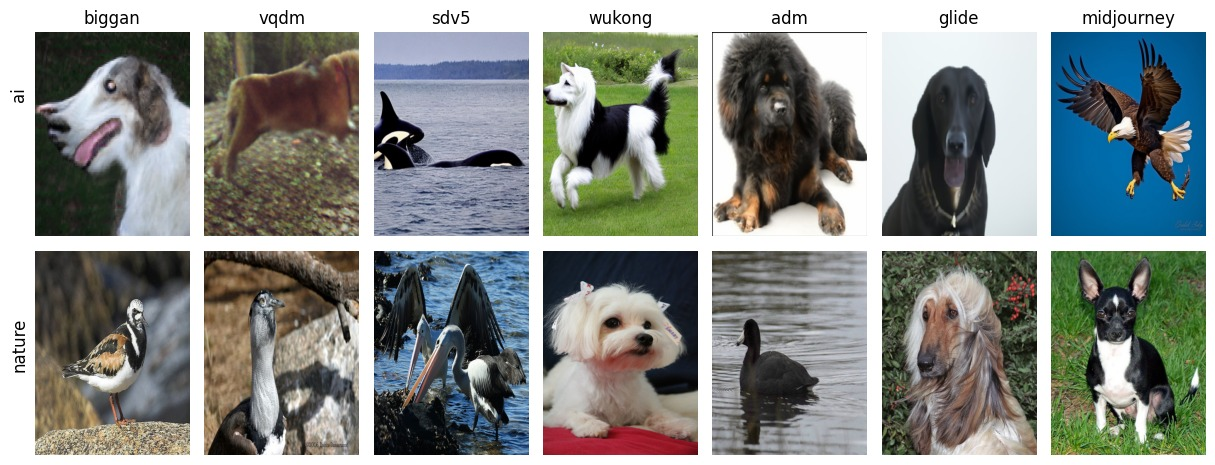
\includegraphics[width=0.8\textwidth]{graphics/dataset_sample.jpeg}
    \caption{Sample images from the GenImage dataset}
    \label{fig:dataset-sample}
\end{figure}


\subsubsection{Augmentation.}
%
% ---- Methodology ----
%
\section{Methodology}

In this paper, we will address the task of classifying images into two categories: images that an AI model and real images generated. For this experiment, we employed a comprehensive approach that involves three different models: a model that uses a custom Convolutional Neural Network (CNN), a pre-trained ResNet model, and a ConvNextSmall network. In this section, we will provide details about the dataset preparation, the network architectures we used, and the evaluation metrics that we used to measure the performance of the three models. 

\subsubsection{Data preparation} As mentioned in a previous section, we used the GenImage dataset that contains several state-of-the-art generative models. The images were separated into different folders, with a training and a validation subfolder, both having two categories: ai and nature. We used all the training and validation images from all the folders, for better training. The images were pre-processed to maintain compatibility with the models, especially with the pre-trained networks, and to standardize input dimensions across the models. We didn't use any data augmentation techniques for this experiment. MODIFICAM DUPA DACA FACEM


\subsubsection{Hardware and software resources} The library employed for the detection of AI synthetic generated images was Keras (maybe link??). For reproducibility purposes, we set the seed to 42. All algorithms in this study were run on Google Colab resources.

\subsubsection{Model Architectures } As mentioned, for this task, we employed three model architectures:  a custom CNN designed specifically for the classification task, a ResNet model fine-tuned from pre-trained weights, and a ConvNextSmall network adapted for binary classification. 

The custom CNN used in this task was designed as a lightweight model, suitable for image classification tasks. We implemented this architecture using TensorFlow and Keras, and it consists of convolutional, pooling, and dense layers, organized to facilitate effective classification. The model uses images of dimensions 32x32x3, and the process begins with three convolutional layers. We use the ReLU(Rectified Linear Unit) activation, padding "Same", that ensures the output dimensions remain consistent with the input, and max-pooling operation, which reduces the spatial dimensions by half, to retain the most salient features. After the convolutional and pooling operations, the output feature maps are flattened into a one-dimensional vector, to prepare them for the dense layers, which consist of 128 neurons with ReLU activation and a dropout layer with a rate of 0.5, to mitigate overfitting by randomly deactivating half of the neurons during training. The output layer is a dense layer with a number of neurons equal to the number of classes (2 classes) and it utilizes a SoftMax activation function. These techniques provide class probabilities for the binary classification task. The model is compiled using an Adam optimizer and we use a categorical cross-entropy loss function.

Resnet50 is a deep CNN architecture that introduced residual learning, a concept that was proposed to solve the vanishing gradient problem in very deep networks. It was developed as part of the ResNet family, and this specific version (ResNet50) became popular and a widely used architecture, especially in image classification. When it comes to fundamental elements, this architecture uses residual blocks, which introduce a shortcut connection, allowing the network to learn residual mappings instead of deep mappings. ResNet50 consists of 50 layers, 48 convolutional layers, 1 max-pooling, and 1 average pooling layer. Another important aspect of this architecture is its parameter number, approximately 25.6 million, a modest number compared to other architectures from the ResNet family. Moreover, the use of bottleneck blocks makes ResNet50 efficient, without losing accuracy points. For our experiment, 
the model was initialized with ImageNet weights to capitalize on pre-learned features, this dataset having over a million images across 1000 categories. This way, our model has a strong baseline of generalized features instead of learning from scratch, like in the first example. The top classification layer of ResNet50 was removed, so we can better adapt the network for our task, to append custom layers for our classification task. Now, the model accepts inputs of 224x224x3, consistent with the ResNet50 architecture. We wanted to ensure that the baseline of the model remained intact, meaning that we wanted the model to keep the generic features. Therefore, we froze the convolutional layers of the base model. This way, the base layers will not be updated during training, saving a lot of computational costs and risk regarding overfitting. A custom classification head is appended to the base model, to fine-tune the base model for our task, a binary classification, consisting of a number of elements: global average pooling, a fully connected layer, which is essentially a dense layer with 256 neurons, and ReLU activation, a dropout layer, with the same scope as the one used in the first experiment with the custom network, where we deactivated half of the neurons and an output layer, a dense layer with a single neuron and sigmoid activation, where the output values closer to 0 indicate AI-generated images, and values closer to 1, real photos. The model was compiled using binary cross-entropy as a loss function, as an optimizer we used Adam, and as a default metric, we selected accuracy. 

ConvNext is a modern architecture, inspired by the design of transformer-based vision models. It was developed by Liu et al. (2022) when the paper "A ConvNet for the 2020s" appeared for the first time and introduced the new generation of models. To summarize, ConvNext tries to combine CNN's performance with the improvements brought by transformers. ConvNextSmall is a lighter version of the ConvNext family, that adopts design choices from the Swin Transformer (Liu et al, 2021), a multi-scale transformer architecture, that is well-designed for high-resolution images in computer vision.  (ONGOING)

%
% ---- Results and discussion ----
%
\section{Results and discussion}

%
% ---- Conclusion ----
%
\section{Conclusion}


%
% ---- Bibliography ----
%
% BibTeX users should specify bibliography style 'splncs04'.
% References will then be sorted and formatted in the correct style.
%
\bibliographystyle{splncs04}
\bibliography{references}

\end{document}
